\chapter{This is the second real chapter}
\graphicspath{{\currfiledir/figures/}}

\lipsum[5-6]

Figure~\ref{fig:seismometer}, shows a standard seismometer that could be used to investigate source parameters of globally recorded earthquakes, such as in \cite{Dziewonski1983}.


\begin{figure}
	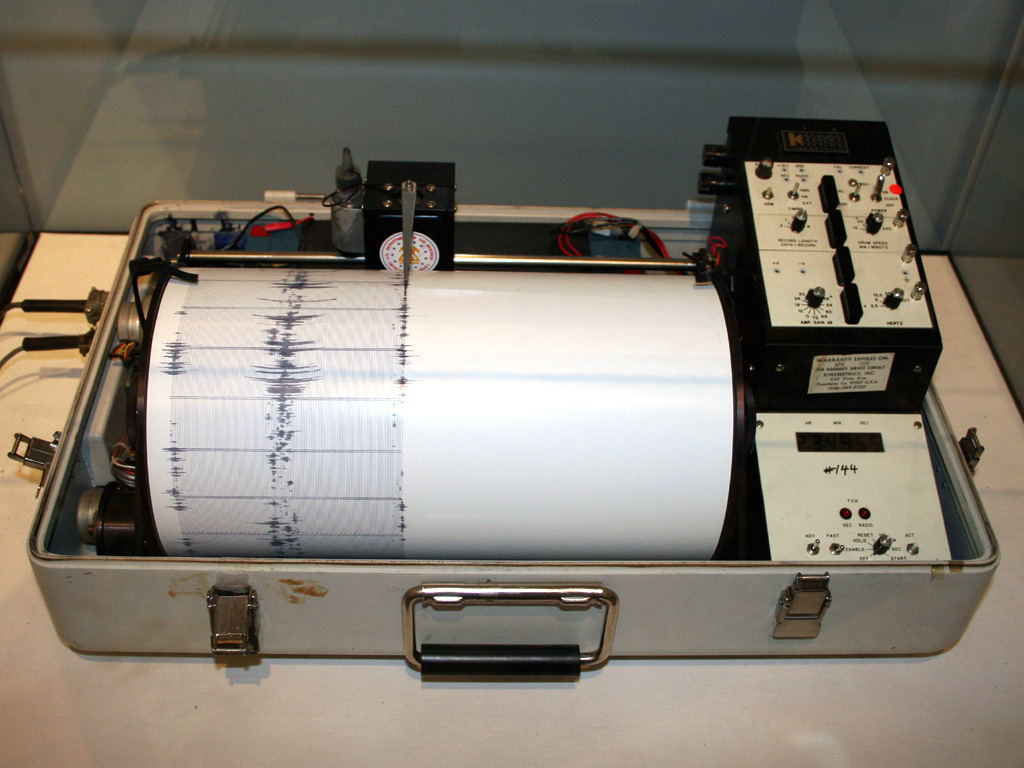
\includegraphics[width=\textwidth]{Kinemetrics_seismograph.jpg}
	\caption{This is Kinemetrics Seismograph, the image was downloaded from the Wikipedia article ``Seismometer'' and the copyright is given by Yamaguchi, CC BY-SA 3.0, \url{https://commons.wikimedia.org/w/index.php?curid=1089235}.}
	\label{fig:seismometer}
\end{figure}

\lipsum[7-8]




\bibliographystyle{unsrt}
\bibliography{bibliography}